\if0
\begin{figure}[hbt!]
    \centering
    \caption{Student online-learning engagement decreased by less for high-income counties after COVID-19}
    \includegraphics[width=0.6\linewidth]{input/timetrend_engagement.eps}
\end{figure}

\begin{figure}[hbt!]
    \caption{COVID-19 was a shock to student and parent behavior with respect to education}
    \centering
    \begin{subfigure}[t]{0.4\textwidth}
    \caption{School-centered resources}
        \centering
        \includegraphics[width=\linewidth]{input/eventstudyplot_specific1_wks.eps}
    \end{subfigure}%
    ~
    \begin{subfigure}[t]{0.4\textwidth}
    \caption{Parent-centered resources}
        \centering
        \includegraphics[width=\linewidth]{input/eventstudyplot_generic_wks.eps}
    \end{subfigure}

    \begin{subfigure}[t]{0.4\textwidth}
    \caption{Student engagement}
        \centering
        \includegraphics[width=\linewidth]{input/eventstudyplot_engagement_wks.eps}
    \end{subfigure}%
    ~
    \begin{subfigure}[t]{0.4\textwidth}
    \caption{Student achievement}
        \centering
        \includegraphics[width=\linewidth]{input/eventstudyplot_badges_wks.eps}
    \end{subfigure}
\end{figure}

\begin{figure}[hbt!]
    \caption{Income inequalities in both parent and student behavior emerged at the onset of the pandemic}
    \centering
    \begin{subfigure}[t]{0.49\textwidth}
    \caption{School-centered resources}
        \centering
        \includegraphics[width=\linewidth]{input/eventstudyplot_specific1_inc.eps}
    \end{subfigure}%
    ~
    \begin{subfigure}[t]{0.49\textwidth}
    \caption{Parent-centered resources}
        \centering
        \includegraphics[width=\linewidth]{input/eventstudyplot_generic_inc.eps}
    \end{subfigure}

    \begin{subfigure}[t]{0.49\textwidth}
    \caption{Student engagement}
        \centering
        \includegraphics[width=\linewidth]{input/eventstudyplot_engagement_inc.eps}
    \end{subfigure}%
    ~
    \begin{subfigure}[t]{0.49\textwidth}
    \caption{Student achievement}
        \centering
        \includegraphics[width=\linewidth]{input/eventstudyplot_badges_inc.eps}
    \end{subfigure}
\end{figure}


\begin{figure}[hbt!]
    \caption{Highly teleworkable areas exhibit the same inequality as high income areas}
    \centering
    \begin{subfigure}[t]{0.49\textwidth}
    \caption{School-centered resources}
        \centering
        \includegraphics[width=\linewidth]{input/eventstudyplot_specific1_tele.eps}
    \end{subfigure}%
    ~
    \begin{subfigure}[t]{0.49\textwidth}
    \caption{Parent-centered resources}
        \centering
        \includegraphics[width=\linewidth]{input/eventstudyplot_generic_tele.eps}
    \end{subfigure}

    \begin{subfigure}[t]{0.49\textwidth}
    \caption{Student engagement}
        \centering
        \includegraphics[width=\linewidth]{input/eventstudyplot_engagement_tele.eps}
    \end{subfigure}%
    ~
    \begin{subfigure}[t]{0.49\textwidth}
    \caption{Student achievement}
        \centering
        \includegraphics[width=\linewidth]{input/eventstudyplot_badges_tele.eps}
    \end{subfigure}
\end{figure}
\fi
\begin{table}[hbtp!]
    \caption{Placebo robustness check: share of households with a computer}
    \label{tab:placebo_computer}
  \centering
  \scalebox{0.99}{
  \begin{tabular}{l c c c c c}
    \toprule
    \input{input/eventstudytable_mtitles.tex} \\
    \midrule
    (A) Post-COVID \\
    \midrule
    \input{input/eventstudytable_wks.tex} \\
    \midrule
    (B) Income Alone \\
    \midrule
    \input{input/eventstudytable_inc.tex} \\
    \midrule
    (C) Computer Alone \\
    \midrule
    \input{input/eventstudytable_comp.tex} \\
    \midrule
    (D) Income + Computer \\
    \midrule
    \input{input/eventstudytable_comptele.tex} \\
    \midrule
    \input{input/eventstudytable_betacomp.tex} \\
    \midrule
    \input{input/eventstudytable_N.tex} \\
    \bottomrule \\
  \end{tabular}
    }
  \begin{minipage}{\textwidth}
      \footnotesize
      \textit{Note}: This table displays the results of eight county level difference-in-differences regressions on the following dependent variables: (1) the natural log of Google Trends search interest for school-centered resources; (2) the natural log of Google Trends search interest parent-centered resources;  (3) Zearn engagement normalized relative to a base period from January 6-February 7,  2020; and (4) Zearn badges normalized relative to a base period from January 6-February 7,  2020. All regression include fixed effects for year and week of year.
      Panel A reveals the first-order effect of COVID-19 on the outcomes.
      Panel B is a difference-in-differences on log income.
      Panel C is a difference-in-differences on the log share of households with a computer.
      Panel D includes both sets of interaction terms.
      I include full interactions, despite not displaying the coefficients on log income and log computer share.
      Note from Eq. \refeq{inctele} that $\gamma$ is the coefficient on Post COVID $\times$ Income, so
      $100 \times \frac{\gamma_B-\gamma_D}{\gamma_B}$ is the percentage change in this coefficient
      when log computer share is included.
      I drop Thanksgiving, Christmas, and New Years, as these are outliers, but the results do not change significantly when they are included.
      I also drop the first three weeks of March, as schools were actively closing during this time.
      Standard errors are in parentheses and clustered by state.
  \end{minipage}


\end{table}

\begin{table}[hbtp!]
    \caption{Placebo robustness check: share of households with a broadband internet connection}
    \label{tab:placebo_internet}
  \centering
  \begin{tabular}{l c c c c c}
    \toprule
    \input{input/eventstudytable_mtitles.tex} \\
    \midrule
    (A) Post-COVID \\
    \midrule
    \input{input/eventstudytable_wks.tex} \\
    \midrule
    (B) Income Alone \\
    \midrule
    \input{input/eventstudytable_inc.tex} \\
    \midrule
    (C) Computer Alone \\
    \midrule
    \input{input/eventstudytable_broad.tex} \\
    \midrule
    (D) Income + Computer \\
    \midrule
    \input{input/eventstudytable_broadtele.tex} \\
    \midrule
    \input{input/eventstudytable_betabroad.tex} \\
    \midrule
    \input{input/eventstudytable_N.tex} \\
    \bottomrule \\
  \end{tabular}
  \begin{minipage}{\textwidth}
      \footnotesize
      \textit{Note}: This table displays the results of eight county level difference-in-differences regressions on the following dependent variables: (1) the natural log of Google Trends search interest for school-centered resources; (2) the natural log of Google Trends search interest parent-centered resources;  (3) Zearn engagement normalized relative to a base period from January 6-February 7,  2020; and (4) Zearn badges normalized relative to a base period from January 6-February 7,  2020. All regression include fixed effects for year and week of year.
      Panel A reveals the first-order effect of COVID-19 on the outcomes.
      Panel B is a difference-in-differences on log income.
      Panel C is a difference-in-differences on the log share of households with broadband internet.
      Panel D includes both sets of interaction terms.
      I include full interactions, despite not displaying the coefficients on log income and log internet.
      Note from Eq. \refeq{inctele} that $\gamma$ is the coefficient on Post COVID $\times$ Income, so
      $100 \times \frac{\gamma_B-\gamma_D}{\gamma_B}$ is the percentage change in this coefficient
      when internet is included.
      I drop Thanksgiving, Christmas, and New Years, as these are outliers, but the results do not change significantly when they are included.
      I also drop the first three weeks of March, as schools were actively closing during this time.
      Standard errors are in parentheses and clustered by state.
  \end{minipage}


\end{table}

\if0
\begin{figure}[hbt!]
    \centering
    \begin{subfigure}[t]{0.65\textwidth}
    \caption{Parent-centered resources}
        \centering
        \includegraphics[width=\linewidth]{input/map_generic.eps}
    \end{subfigure}%

    \begin{subfigure}[t]{0.65\textwidth}
    \caption{School-centered resources}
        \centering
        \includegraphics[width=\linewidth]{input/map_specific1.eps}
    \end{subfigure}
\end{figure}


\begin{figure}[hbt!]
    \centering
    \begin{subfigure}[t]{0.65\textwidth}
    \caption{Zearn engagement}
        \centering
        \includegraphics[width=\linewidth]{input/map_engagement.eps}
    \end{subfigure}%

    \begin{subfigure}[t]{0.65\textwidth}
    \caption{Zearn badges}
        \centering
        \includegraphics[width=\linewidth]{input/map_badges.eps}
    \end{subfigure}
\end{figure}

\begin{figure}[hbt!]
    \centering
    \begin{subfigure}[t]{0.65\textwidth}
    \caption{Share of households with broadband internet}
        \centering
        \includegraphics[width=\linewidth]{input/map_broad.eps}
    \end{subfigure}%

    \begin{subfigure}[t]{0.65\textwidth}
    \caption{Share of households with computer}
        \centering
        \includegraphics[width=\linewidth]{input/map_comp.eps}
    \end{subfigure}
\end{figure}

\begin{figure}[hbt!]
    \centering
    \begin{subfigure}[t]{0.65\textwidth}
    \caption{Teleworkability share}
        \centering
        \includegraphics[width=\linewidth]{input/map_tele.eps}
    \end{subfigure}%

    \begin{subfigure}[t]{0.65\textwidth}
    \caption{Work from home score}
        \centering
        \includegraphics[width=\linewidth]{input/map_wfhscore.eps}
    \end{subfigure}
\end{figure}

\begin{figure}[hbt!]
    \centering
    \begin{subfigure}[t]{0.75\textwidth}
    \caption{Student achievement}
        \centering
        \includegraphics[width=\linewidth]{input/eventstudyplot_badges_inccomp_long.eps}
    \end{subfigure}%
\end{figure}

\begin{figure}[hbt!]
    \centering
    \begin{subfigure}[t]{0.75\textwidth}
    \caption{Student achievement}
        \centering
        \includegraphics[width=\linewidth]{input/eventstudyplot_badges_incbroad_long.eps}
    \end{subfigure}%
\end{figure}
\fi

\if0
\begin{figure}[hbt!]
    \caption{\cite{bh1} Replication: COVID-19 is a shock search interest}
    \centering
    \begin{subfigure}[t]{0.45\textwidth}
    \caption{School-centered}
        \centering
        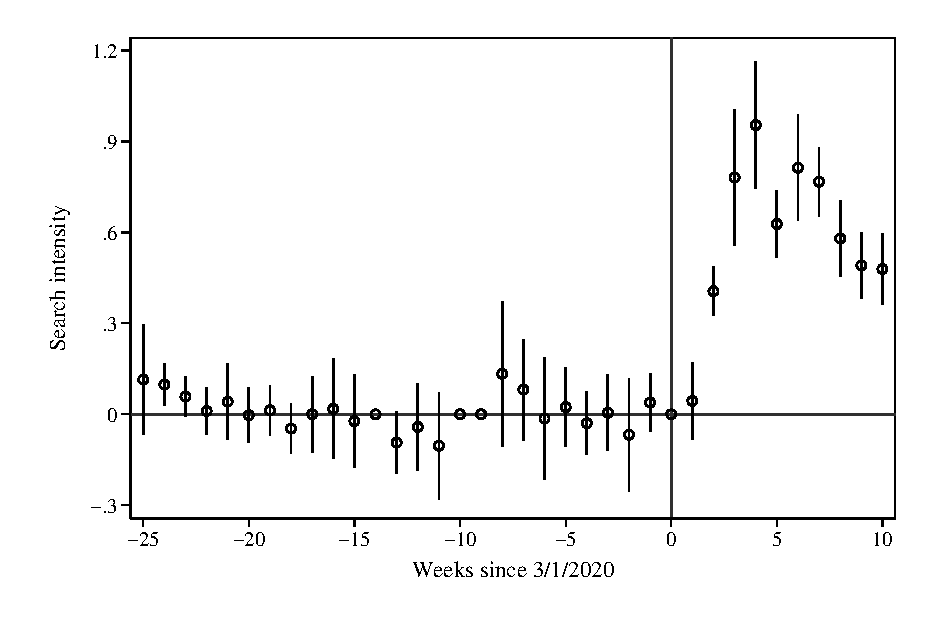
\includegraphics[width=\linewidth]{input/intensity_bh_replication_event_study_specific1.eps}
    \end{subfigure}%
    ~
    \begin{subfigure}[t]{0.45\textwidth}
    \caption{Parent-centered}
        \centering
        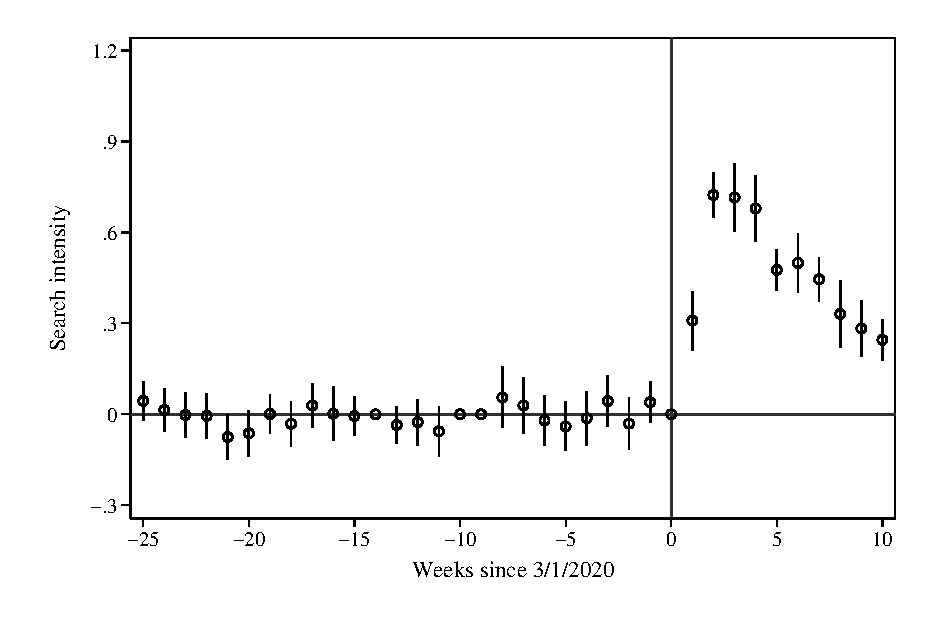
\includegraphics[width=\linewidth]{input/intensity_bh_replication_event_study_generic.eps}
    \end{subfigure}
    \caption{This widened the high-low SES search interest gap}
      \centering
      \begin{subfigure}[t]{0.45\textwidth}
      \caption{School-centered}
          \centering
          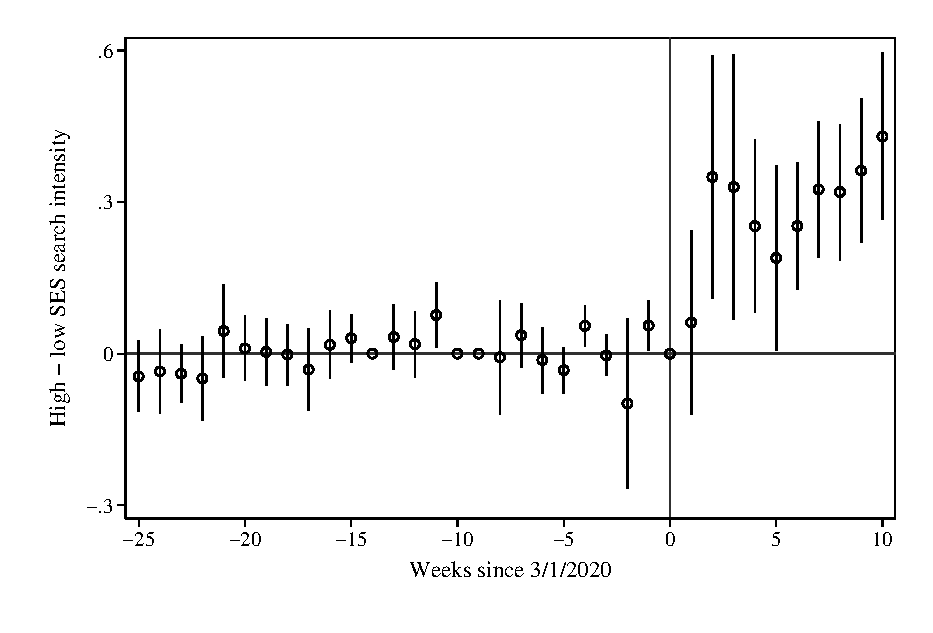
\includegraphics[width=\linewidth]{input/ses_bh_replication_event_study_specific1.eps}
      \end{subfigure}%
      ~
      \begin{subfigure}[t]{0.45\textwidth}
      \caption{Parent-centered}
          \centering
          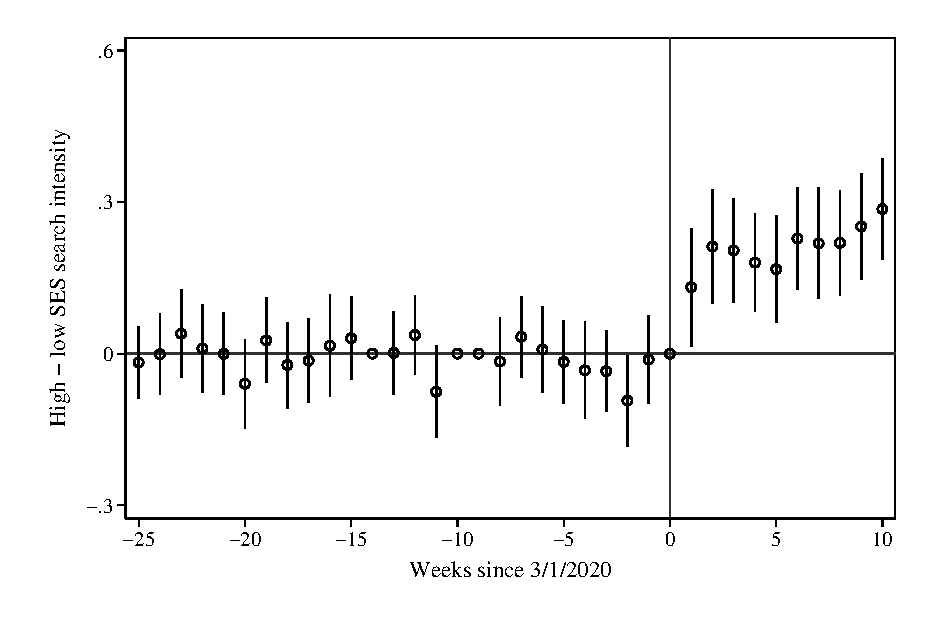
\includegraphics[width=\linewidth]{input/ses_bh_replication_event_study_generic.eps}
      \end{subfigure}
\begin{minipage}{\linewidth}
\footnotesize    \textit{Note:} This replicates DMA-level regressions from \cite{bh1}. I employ similar methodology in \ref{fig:eventstudy} and related appendix figures from the county-level. Panels (a) and (b) regress search interest on an indicator for relative week since March 1, 2020. Panels (c) and (d) are event studies by high-low SES group, defined by above or below median. SES is determined by taking the first principal component of income, broadband internet access, and presence of computer. All regressions include school year and week of year fixed effects. Intervals are 95\% confidence intervals and standard errors are clustered by state.
\end{minipage}
\end{figure}

\begin{table}[htbp] \centering
\def\sym#1{\ifmmode^{#1}\else\(^{#1}\)\fi}
\caption{\cite{bh1} Replication: Changes in Search Intensity}
\scalebox{0.8}{
\begin{tabular*}{1\textwidth}{@{\extracolsep{\fill}}l*{4}{c}}
\toprule
&School-       &Parent-        &                       &               \\
&centered      &centered       &Google         &Khan   \\
&resources     &resources      &Classroom      &Academy\\
&(1)&(2)&(3)&(4)\\
\midrule
(A) Nationwide \\
\cmidrule{1-1}
Post COVID        &        0.51\sym{***}&        0.34\sym{***}&        0.76\sym{***}&        0.41\sym{***}\\
                    &      (0.05)         &      (0.02)         &      (0.05)         &      (0.03)         \\
\cmidrule{1-1}
(B) By median SES\\
\cmidrule{1-1}
Post COVID $\times$ Low-SES&        0.31\sym{***}&        0.22\sym{***}&        0.59\sym{***}&        0.32\sym{***}\\
                    &      (0.05)         &      (0.02)         &      (0.07)         &      (0.03)         \\
High SES            &        0.02         &        0.01         &        0.10         &        0.05         \\
                    &      (0.06)         &      (0.05)         &      (0.10)         &      (0.05)         \\
Post COVID $\times$ High-SES&        0.39\sym{***}&        0.24\sym{***}&        0.33\sym{***}&        0.19\sym{***}\\
                    &      (0.11)         &      (0.03)         &      (0.11)         &      (0.05)         \\
                    &                     &                     &                     &                     \\
\cmidrule{1-1}
(C) By income, online access, race\\
\cmidrule{1-1}
Post COVID $\times$ HH mean income&        0.14\sym{***}&        0.08\sym{***}&        0.12\sym{***}&        0.07\sym{***}\\
                    &      (0.04)         &      (0.01)         &      (0.03)         &      (0.02)         \\
                    &                     &                     &                     &                     \\
Post COVID $\times$ \% of HH w/ broadband&        0.36\sym{***}&        0.30\sym{***}&        0.31\sym{***}&        0.27\sym{***}\\
                    &      (0.08)         &      (0.03)         &      (0.09)         &      (0.04)         \\
                    &                     &                     &                     &                     \\
Post COVID $\times$ \% of HH w/ computer&        0.44\sym{***}&        0.41\sym{***}&        0.41\sym{***}&        0.33\sym{***}\\
                    &      (0.10)         &      (0.04)         &      (0.10)         &      (0.07)         \\
                    &                     &                     &                     &                     \\
Post COVID $\times$ \% of schools in rural area&       -0.16\sym{***}&       -0.08\sym{***}&       -0.18\sym{***}&       -0.09\sym{***}\\
                    &      (0.03)         &      (0.01)         &      (0.03)         &      (0.02)         \\
                    &                     &                     &                     &                     \\
Post COVID $\times$ \% of students Black&       -0.09\sym{***}&       -0.06\sym{***}&       -0.03         &       -0.06\sym{***}\\
                    &      (0.03)         &      (0.01)         &      (0.04)         &      (0.02)         \\
                    &                     &                     &                     &                     \\
\midrule
& 50400 & 50400 & 50400 & 50400
\end{tabular*}
}
\begin{minipage}{\textwidth}
\footnotesize    \textit{Note:} This replicates DMA-level regressions from \cite{bh1}. The outcomes are in log Google Trends search interest, where (1) and (2) are groupings of terms and (3) and (4) are specific terms. Post-COVID is after March 1, 2020. Panel (A) reveals that COVID-19 is a shock to search interest for resources. Panel (B) shows the results is a difference in differences regression on high-low SES, defined by the median. Panel (C) regresses on each of the individual factors that contribute to SES.
\end{minipage}
\end{table}

\begin{table}[htbp] \centering
\def\sym#1{\ifmmode^{#1}\else\(^{#1}\)\fi}
\caption{Changes in Search Intensity, excluding low search intensity observations}
\scalebox{0.7}{
\begin{tabular*}{1\textwidth}{@{\extracolsep{\fill}}l*{4}{c}}
\midrule
&School-       &Parent-        &                       &               \\
&centered      &centered       &Google         &Khan   \\
&resources     &resources      &Classroom      &Academy\\
&(1)&(2)&(3)&(4)\\
\midrule
(A) Nationwide \\
\cmidrule{1-1}
Post COVID        &        0.52\sym{***}&        0.35\sym{***}&        0.76\sym{***}&        0.41\sym{***}\\
                    &      (0.05)         &      (0.02)         &      (0.05)         &      (0.03)         \\
\cmidrule{1-1}
(B) By median SES\\
\cmidrule{1-1}
Post COVID $\times$ Low-SES&        0.30\sym{***}&        0.21\sym{***}&        0.59\sym{***}&        0.30\sym{***}\\
                    &      (0.05)         &      (0.02)         &      (0.07)         &      (0.03)         \\
High SES            &       -0.04         &       -0.12\sym{***}&        0.07         &        0.01         \\
                    &      (0.06)         &      (0.03)         &      (0.10)         &      (0.06)         \\
Post COVID $\times$ High-SES&        0.44\sym{***}&        0.27\sym{***}&        0.35\sym{***}&        0.21\sym{***}\\
                    &      (0.10)         &      (0.03)         &      (0.11)         &      (0.05)         \\
                    &                     &                     &                     &                     \\
\cmidrule{1-1}
(C) By income, online access, race\\
\cmidrule{1-1}
Post COVID $\times$ household mean income&        0.15\sym{***}&        0.09\sym{***}&        0.13\sym{***}&        0.08\sym{***}\\
                    &      (0.03)         &      (0.01)         &      (0.03)         &      (0.02)         \\
                    &                     &                     &                     &                     \\
Post COVID $\times$ \% of households with broadband&        0.43\sym{***}&        0.34\sym{***}&        0.36\sym{***}&        0.30\sym{***}\\
                    &      (0.08)         &      (0.03)         &      (0.09)         &      (0.05)         \\
                    &                     &                     &                     &                     \\
Post COVID $\times$ \% of households with a computer&        0.54\sym{***}&        0.46\sym{***}&        0.47\sym{***}&        0.38\sym{***}\\
                    &      (0.10)         &      (0.04)         &      (0.10)         &      (0.07)         \\
                    &                     &                     &                     &                     \\
Post COVID $\times$ \% of schools in rural area&       -0.18\sym{***}&       -0.10\sym{***}&       -0.19\sym{***}&       -0.10\sym{***}\\
                    &      (0.03)         &      (0.01)         &      (0.03)         &      (0.02)         \\
                    &                     &                     &                     &                     \\
Post COVID $\times$ \% of students black&       -0.09\sym{***}&       -0.04\sym{***}&       -0.02         &       -0.06\sym{***}\\
                    &      (0.03)         &      (0.02)         &      (0.04)         &      (0.02)         \\
                    &                     &                     &                     &                     \\
\hline
& 45845 & 40829 & 45682 & 44240
\end{tabular*}
}
\end{table}


\begin{figure}[hbt!]
  \caption{Student online-learning engagement decreased by less in high-income counties after COVID-19}
    \centering
    \includegraphics[width=0.6\linewidth]{input/timetrend_engagement.eps}
    \begin{minipage}{\textwidth}
        \footnotesize
        \textit{Note:} This figure shows the trend in mean county-level standardized Zearn engagement
        split by quintile, with the middle three quintiles grouped.
        I drop the weeks containing Thanksgiving, Christmas, and New Years,
        as they are outliers.
    \end{minipage}
\end{figure}
\fi
